%
% slides.tex
%
% (c) 2019 Prof Dr Andreas Müller, Hochschule Rapperswil
%

\begin{document}

\theoremstyle{definition}
\newtheorem{signal}{Signal}
\newtheorem{abgetastet}{Abgetastetes Signal}
\newtheorem{skalar}{Skalarprodukt und Norm}
\newtheorem{cauchyschwarz}{Cauchy-Schwarz-Ungleichung}
\newtheorem{nachteile}{Nachteile}
\newtheorem{idee}{Idee}
\newtheorem{faktoren}{Erfolgsfaktoren}

\ifthenelse{\boolean{presentation}}{
\begin{frame}
\titlepage
\end{frame}
}{}

%
% Vergleich von Binärsignalen
%
\begin{frame}
\frametitle{Vergleich von Binärsignalen}
\centering
\def\achsen{
	\draw[->,line width=0.7pt] (-0.1,0)--(11.5,0) coordinate[label={$t$}];
	\draw[->,line width=0.7pt] (0,-1.1)--(0,1.4);
	\draw[line width=0.7pt] (-0.1,-1)--(0.1,-1);
	\node at (-0.1,-1) [left] {$-1$};
	\draw[line width=0.7pt] (-0.1,1)--(0.1,1);
	\node at (-0.1,1) [left] {$1$};
	\foreach \i in {1,...,11}{
		\draw[line width=0.7pt] ({\i},-0.1)--({\i},0.1);
	}
}
\begin{tikzpicture}[>=latex]

\begin{scope}[yshift=3cm]
\achsen
\node at (-0.1,0) [left] {$f$};
\uncover<1->{
	\draw[line width=1pt,color=red] (1,0)--(1,1);
	\fill[color=red] (1,1) circle[radius=0.08];
}
\uncover<2->{
	\draw[line width=1pt,color=red] (2,0)--(2,1);
	\fill[color=red] (2,1) circle[radius=0.08];
}
\uncover<3->{
	\draw[line width=1pt,color=red] (3,0)--(3,-1);
	\fill[color=red] (3,-1) circle[radius=0.08];
}
\uncover<4->{
	\draw[line width=1pt,color=red] (4,0)--(4,1);
	\fill[color=red] (4,1) circle[radius=0.08];
}
\uncover<5->{
	\draw[line width=1pt,color=red] (5,0)--(5,-1);
	\fill[color=red] (5,-1) circle[radius=0.08];
}
\uncover<6->{
	\draw[line width=1pt,color=red] (6,0)--(6,1);
	\fill[color=red] (6,1) circle[radius=0.08];
}
\uncover<7->{
	\draw[line width=1pt,color=red] (7,0)--(7,1);
	\fill[color=red] (7,1) circle[radius=0.08];
}
\uncover<8->{
	\draw[line width=1pt,color=red] (8,0)--(8,1);
	\fill[color=red] (8,1) circle[radius=0.08];
}
\uncover<9->{
	\draw[line width=1pt,color=red] (9,0)--(9,-1);
	\fill[color=red] (9,-1) circle[radius=0.08];
}
\uncover<10->{
	\draw[line width=1pt,color=red] (10,0)--(10,1);
	\fill[color=red] (10,1) circle[radius=0.08];
}
\uncover<11->{
	\draw[line width=1pt,color=red] (11,0)--(11,1);
	\fill[color=red] (11,1) circle[radius=0.08];
}
\end{scope}

\begin{scope}
\achsen
\node at (-0.1,0) [left] {$g$};
\uncover<1->{
	\draw[line width=1pt,color=blue] (1,0)--(1,1);
	\fill[color=blue] (1,1) circle[radius=0.08];
}
\uncover<2->{
	\draw[line width=1pt,color=blue] (2,0)--(2,-1);
	\fill[color=blue] (2,-1) circle[radius=0.08];
}
\uncover<3->{
	\draw[line width=1pt,color=blue] (3,0)--(3,1);
	\fill[color=blue] (3,1) circle[radius=0.08];
}
\uncover<4->{
	\draw[line width=1pt,color=blue] (4,0)--(4,-1);
	\fill[color=blue] (4,-1) circle[radius=0.08];
}
\uncover<5->{
	\draw[line width=1pt,color=blue] (5,0)--(5,1);
	\fill[color=blue] (5,1) circle[radius=0.08];
}
\uncover<6->{
	\draw[line width=1pt,color=blue] (6,0)--(6,-1);
	\fill[color=blue] (6,-1) circle[radius=0.08];
}
\uncover<7->{
	\draw[line width=1pt,color=blue] (7,0)--(7,1);
	\fill[color=blue] (7,1) circle[radius=0.08];
}
\uncover<8->{
	\draw[line width=1pt,color=blue] (8,0)--(8,-1);
	\fill[color=blue] (8,-1) circle[radius=0.08];
}
\uncover<9->{
	\draw[line width=1pt,color=blue] (9,0)--(9,1);
	\fill[color=blue] (9,1) circle[radius=0.08];
}
\uncover<10->{
	\draw[line width=1pt,color=blue] (10,0)--(10,-1);
	\fill[color=blue] (10,-1) circle[radius=0.08];
}
\uncover<11->{
	\draw[line width=1pt,color=blue] (11,0)--(11,1);
	\fill[color=blue] (11,1) circle[radius=0.08];
}
\end{scope}

\begin{scope}[yshift=-2cm]
\node at (0.4,0) [left] {$f_kg_k$};
\node at (0.4,-0.7) [left] {$\sum f_kg_k$};
\uncover<1->{
	\node at (1,0) {$+1$};
	\node at (1,-0.7) {$1$};
}
\uncover<2->{
	\node at (2,0) {$-1$};
	\node at (2,-0.7) {$0$};
}
\uncover<3->{
	\node at (3,0) {$-1$};
	\node at (3,-0.7) {$-1$};
}
\uncover<4->{
	\node at (4,0) {$-1$};
	\node at (4,-0.7) {$-2$};
}
\uncover<5->{
	\node at (5,0) {$-1$};
	\node at (5,-0.7) {$-3$};
}
\uncover<6->{
	\node at (6,0) {$-1$};
	\node at (6,-0.7) {$-4$};
}
\uncover<7->{
	\node at (7,0) {$+1$};
	\node at (7,-0.7) {$-3$};
}
\uncover<8->{
	\node at (8,0) {$-1$};
	\node at (8,-0.7) {$-4$};
}
\uncover<9->{
	\node at (9,0) {$-1$};
	\node at (9,-0.7) {$-5$};
}
\uncover<10->{
	\node at (10,0) {$-1$};
	\node at (10,-0.7) {$-6$};
}
\uncover<11->{
	\node at (11,0) {$+1$};
	\node at (11,-0.7) {$-5$};
}
\end{scope}

\end{tikzpicture}
\end{frame}

%
% Vergleich von Funktionen
%
\def\vergleich#1{
\begin{frame}
\frametitle{Funktionsvergleich}
\centering
\includegraphics[width=\hsize]{#1}
\end{frame}
}

\vergleich{../../buch/chapters/1-geometrie/images/sinsin.pdf}
\vergleich{../../buch/chapters/1-geometrie/images/sincos.pdf}
\vergleich{../../buch/chapters/1-geometrie/images/sinrect.pdf}
\vergleich{../../buch/chapters/1-geometrie/images/cosrect.pdf}
\vergleich{../../buch/chapters/1-geometrie/images/sinrand.pdf}

\begin{frame}
\frametitle{Skalarprodukt von abgetasteten Signalen}
\begin{signal}
Funktion $\mathbb R \to \mathbb R$:
\[
t\mapsto f(t)
\]
\end{signal}

Abtastung: Auswertung an Stellen $t_k = hk$, $h=\text{Abtastinterval}$,
$k\in\mathbb Z$, ergibt $f_k=f(t_k)$

\pause

\begin{abgetastet}
Funktion $\mathbb Z\to \mathbb R: k\mapsto f_k $
\end{abgetastet}

\pause

\begin{skalar}
Mass für Ähnlichkeit:
\[
\langle x,y\rangle
=
\langle x_k, y_k \rangle
=
\sum_{k\in\mathbb Z} x_ky_k
\qquad
\|x\|^2 = \langle x,x\rangle = \sum_{k\in\mathbb Z} |x_k|^2
\]
\end{skalar}

\end{frame}

%
% Geometrische Intuition für das Skalarprodukt
%
\begin{frame}
\frametitle{Geometrie}
\begin{cauchyschwarz}
\[
|\langle x,y\rangle| \le \sqrt{\langle x,x\rangle \cdot \langle y,y\rangle}
= \|x\|\cdot \|y\|
\]
Gleichheit genau dann, wenn $x$ und $y$ linear abhängig sind.
\end{cauchyschwarz}

\pause
Masszahl für ``Ähnlichkeit'' von Signalen:
\[
-1 \le \frac{\langle x,y\rangle}{\|x\|\cdot \|y\|}\le 1
\]
\begin{itemize}
\item
Nahe bei $\pm 1$: ähnlich
\item
Gleichheit genau dann, wenn $x$ und $y$ Vielfache voneinander
\end{itemize}
$\Rightarrow$ Vektorgeometrie für Signale, Orthonormalbasis
\end{frame}

%
% Fourier-Idee
%
\begin{frame}
\frametitle{Fourier-Idee}
\begin{idee}
Vergleich mit $\sin(\omega t)$ und $\cos(\omega t)$ für beliebige Frequenzen
$\omega\in\mathbb R$.
\end{idee}
\bigskip

Fourier-Koeffizienten:
\[
\langle \sin(\omega t), f(t) \rangle
\qquad\text{und}\qquad
\langle \cos(\omega t), f(t) \rangle
\]

\bigskip

\begin{nachteile}
\begin{enumerate}[<+->]
\item
$\sin(t + 2\pi) = \sin(t)$
$\Rightarrow$ 
das um $2\pi$ zeitverschobene Signal liefert den gleichen
Fourier-Koeffizienten
\item
Fourierkoeffizient $\langle \sin t, f\rangle$ sagt nichts darüber aus, wo
$f$ ``interessant'' ist
\item
Fourier-Transformation kann erst bestimmt werden, wenn das ganze Signal
``vorbei'' ist.
\end{enumerate}
\end{nachteile}
\end{frame}

%
% Wavelet-Idee
%
\begin{frame}
\frametitle{Wavelet-Idee}
\begin{idee}
Signal vergleichen mit kurzen Wellenstückchen: ``Wavelets''
\end{idee}
\pause
\begin{faktoren}
\begin{itemize}[<+->]
\item 
``Gute'' Wavelets, vergleichbar mit realistischen Signalen
\uncover<6->{
{\color{red}
$\rightarrow$
Gabor-Wavelet,
Mexikanerhut,
Meyer-Wavelet,
Daubechies-Wavelets, Coifflet,
Symlet, \dots}
}
\item 
Schneller Berechnungsalgorithmus
\uncover<7->{
{\color{red}
$\rightarrow$
Multiskalen-Analyse,
Wavelets mit kompaktem Träger}
}
\item 
Schneller Synthesealgorithmus
\item 
orthonormierte Basis
\uncover<8->{
{\color{red}
$\rightarrow$ Frame, Multiskalen-Analyse}
}
\end{itemize}
\end{faktoren}
\end{frame}

%
% Mexikanerhut-Wavelet
%
\begin{frame}
\frametitle{Mexikanerhut}
\centering
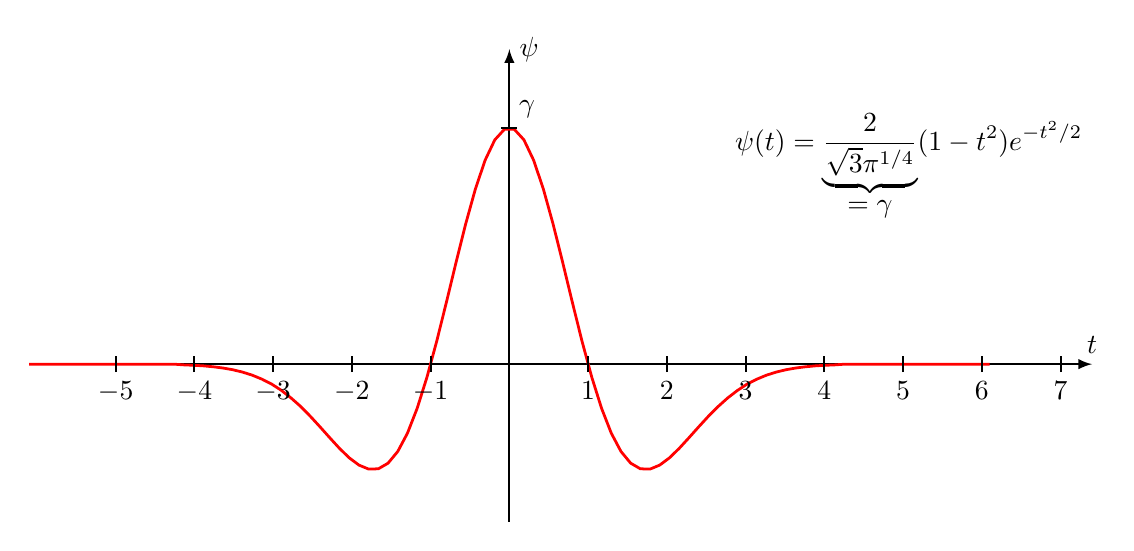
\begin{tikzpicture}[>=latex]
\draw[->,line width=0.7pt] (-5.1,0)--(7.4,0) coordinate[label=$t$];
\draw[->,line width=0.7pt] (0,-2)--(0,4) coordinate[label={right:$\psi$}];
\draw[line width=1pt,color=red] plot[domain=-6.1:6.1,samples=100]
	({\x},{3*(1-\x*\x)*exp(-\x*\x/2)});
\foreach \x in{1,...,7}{
	\draw[line width=0.7pt] ({\x},-0.1)--({\x},0.1);
	\node at ({\x},-0.1) [below] {$\x$};
}
\foreach \x in{1,...,5}{
	\draw[line width=0.7pt] ({-\x},-0.1)--({-\x},0.1);
	\node at ({-\x},-0.1) [below] {$-\x$};
}
\node at (7.4,2.5) [left] {$\psi(t) = \displaystyle\underbrace{\frac{2}{\sqrt{3}\pi^{1/4}}}_{\displaystyle=\gamma} (1-t^2)e^{-t^2/2}$};
\node at (0,3) [above right] {$\gamma$};
\draw[line width=1pt] (-0.1,3)--(0.1,3);
\end{tikzpicture}
\end{frame}

%
% Analyse mit Mexikanerhut
%
\begin{frame}
\frametitle{Analyse mit Mexikanerhut}
\centering
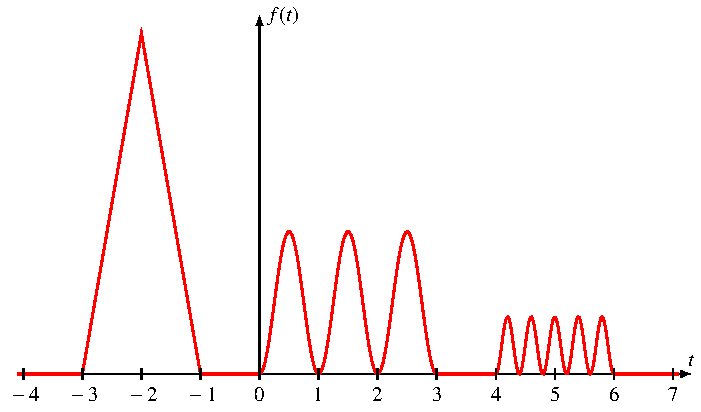
\includegraphics[width=\hsize]{../../buch/chapters/4-cwt/images/f.pdf}
\end{frame}

\begin{frame}
\frametitle{Analyse mit Mexikanerhut}
\centering
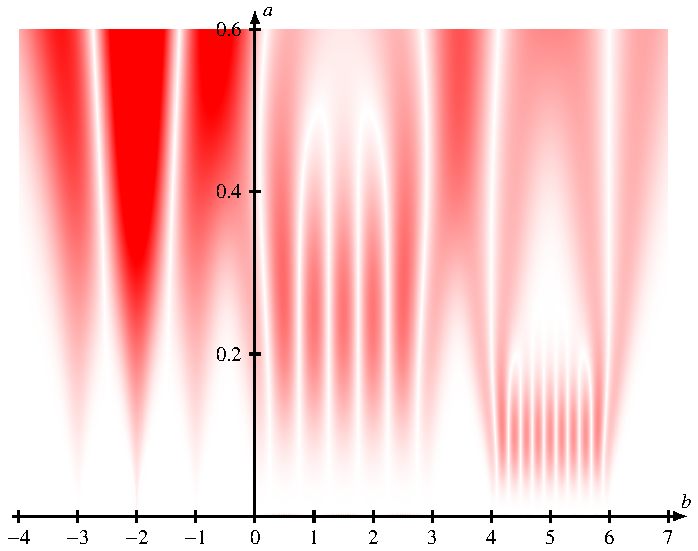
\includegraphics[width=0.73\hsize]{../../buch/chapters/4-cwt/images/notes.pdf}
\end{frame}

%
% Stueckweise konstante Funktionen
%
\def\stueck#1{
\begin{frame}
\frametitle{Stückweise konstante Funktionen}
\centering
\includegraphics[width=\hsize]{#1}
\end{frame}
}

\stueck{../../buch/chapters/3-haar/images/stueckweise1.pdf}
\stueck{../../buch/chapters/3-haar/images/stueckweise8.pdf}
\stueck{../../buch/chapters/3-haar/images/stueckweise64.pdf}

%
% Haar-Vaterwavelet
%
\begin{frame}
\frametitle{Haar-Vater-Wavelet}
\centering
\begin{tikzpicture}[>=latex]

\only<1>{
\node at (2,1) [above] {$\varphi$};
\fill[color=blue!10] (0,0)--(4,0)--(4,1)--(0,1)--cycle;
\draw[line width=1pt,color=blue] (-0.1,0)--(0,0);
\draw[line width=0.1pt,color=blue] (0,0)--(0,1);
\draw[line width=1pt,color=blue] (0,1)--(4,1);
\draw[line width=0.1pt,color=blue] (4,0)--(4,1);
\draw[line width=1pt,color=blue] (4,0)--(12.1,0);
}
\only<2>{
\node at (6,1) [above] {$T_1\varphi$};
\fill[color=blue!10] (4,0)--(8,0)--(8,1)--(4,1)--cycle;
\draw[line width=1pt,color=blue] (-0.1,0)--(4,0);
\draw[line width=0.1pt,color=blue] (4,0)--(4,1);
\draw[line width=1pt,color=blue] (4,1)--(8,1);
\draw[line width=0.1pt,color=blue] (8,0)--(8,1);
\draw[line width=1pt,color=blue] (8,0)--(12.1,0);
}
\only<3>{
\node at (10,1) [above] {$T_2\varphi$};
\fill[color=blue!10] (8,0)--(12,0)--(12,1)--(8,1)--cycle;
\draw[line width=1pt,color=blue] (-0.1,0)--(8,0);
\draw[line width=0.1pt,color=blue] (8,0)--(8,1);
\draw[line width=1pt,color=blue] (8,1)--(12,1);
\draw[line width=0.1pt,color=blue] (12,0)--(12,1);
\draw[line width=1pt,color=blue] (12,0)--(12.1,0);
}
\only<4>{
\node at (1,{sqrt(2)}) [above] {$D_{\frac12}\varphi$};
\fill[color=blue!10] (0,0)--(2,0)--(2,{sqrt(2)})--(0,{sqrt(2)})--cycle;
\draw[line width=1pt,color=blue] (-0.1,0)--(0,0);
\draw[line width=0.1pt,color=blue] (0,0)--(0,{sqrt(2)});
\draw[line width=1pt,color=blue] (0,{sqrt(2)})--(2,{sqrt(2)});
\draw[line width=0.1pt,color=blue] (2,0)--(2,{sqrt(2)});
\draw[line width=1pt,color=blue] (2,0)--(12.1,0);
}
\only<5>{
\node at (0.5,{2}) [above] {$D_{\frac12}\varphi$};
\fill[color=blue!10] (0,0)--(1,0)--(1,{2})--(0,{2})--cycle;
\draw[line width=1pt,color=blue] (-0.1,0)--(0,0);
\draw[line width=0.1pt,color=blue] (0,0)--(0,{2});
\draw[line width=1pt,color=blue] (0,{2})--(1,{2});
\draw[line width=0.1pt,color=blue] (1,0)--(1,{2});
\draw[line width=1pt,color=blue] (1,0)--(12.1,0);
}

\draw[->,line width=0.7pt] (-0.1,0)--(12.4,0) coordinate[label={$t$}];
\draw[->,line width=0.7pt] (0,-0.1)--(0,2.3) coordinate[label={left:$\varphi$}];

\foreach \x in {1,...,3}{
	\draw[line width=0.7pt] ({4*\x},-0.1)--({4*\x},0.1);
	\node at ({4*\x},-0.1) [below] {$\x$};
}
\draw[line width=0.7pt] (-0.1,1)--(0.1,1);
\node at (-0.1,1) [left] {$1$};

\end{tikzpicture}
\end{frame}

%
% Haar-Mutterwavelet
%
\begin{frame}
\frametitle{Haar-Mutter-Wavelet}
\centering
\begin{tikzpicture}[>=latex]

\only<1,7->{
\node at (2,1) [above] {$\psi$};
\fill[color=red!10] (0,0)--(0,1)--(2,1)--(2,-1)--(4,-1)--(4,0)--cycle;
\draw[line width=1pt,color=red] (-0.1,0)--(0,0);
\draw[line width=0.1pt,color=red] (0,0)--(0,1);
\draw[line width=1pt,color=red] (0,1)--(2,1);
\draw[line width=0.1pt,color=red] (2,1)--(2,-1);
\draw[line width=1pt,color=red] (2,-1)--(4,-1);
\draw[line width=0.1pt,color=red] (4,-1)--(4,0);
\draw[line width=1pt,color=red] (4,0)--(12.1,0);
}
\only<2>{
\node at (6,1) [above] {$T_1\psi$};
\fill[color=red!10] (4,0)--(4,1)--(6,1)--(6,-1)--(8,-1)--(8,0)--cycle;
\draw[line width=1pt,color=red] (-0.1,0)--(4,0);
\draw[line width=0.1pt,color=red] (4,0)--(4,1);
\draw[line width=1pt,color=red] (4,1)--(6,1);
\draw[line width=0.1pt,color=red] (6,1)--(6,-1);
\draw[line width=1pt,color=red] (6,-1)--(8,-1);
\draw[line width=0.1pt,color=red] (8,-1)--(8,0);
\draw[line width=1pt,color=red] (8,0)--(12.1,0);
}
\only<3>{
\node at (10,1) [above] {$T_2\psi$};
\fill[color=red!10] (8,0)--(8,1)--(10,1)--(10,-1)--(12,-1)--(12,0)--cycle;
\draw[line width=1pt,color=red] (-0.1,0)--(8,0);
\draw[line width=0.1pt,color=red] (8,0)--(8,1);
\draw[line width=1pt,color=red] (8,1)--(10,1);
\draw[line width=0.1pt,color=red] (10,1)--(10,-1);
\draw[line width=1pt,color=red] (10,-1)--(12,-1);
\draw[line width=0.1pt,color=red] (12,-1)--(12,0);
\draw[line width=1pt,color=red] (12,0)--(12.1,0);
}
\only<4>{
\node at (1,{sqrt(2)}) [above] {$D_{\frac12}\psi$};
\fill[color=red!10] (0,0)--(0,{sqrt(2)})--(1,{sqrt(2)})--(1,-{sqrt(2)})--(2,-{sqrt(2)})--(2,0)--cycle;
\draw[line width=1pt,color=red] (-0.1,0)--(0,0);
\draw[line width=0.1pt,color=red] (0,0)--(0,{sqrt(2)});
\draw[line width=1pt,color=red] (0,{sqrt(2)})--(1,{sqrt(2)});
\draw[line width=0.1pt,color=red] (1,{sqrt(2)})--(1,{-sqrt(2)});
\draw[line width=1pt,color=red] (1,{-sqrt(2)})--(2,{-sqrt(2)});
\draw[line width=0.1pt,color=red] (2,{-sqrt(2)})--(2,0);
\draw[line width=1pt,color=red] (2,0)--(12.1,0);
}
\only<5>{
\node at (3,{sqrt(2)}) [above] {$T_{\frac12}D_{\frac12}\psi$};
\fill[color=red!10] (2,0)--(2,{sqrt(2)})--(3,{sqrt(2)})--(3,-{sqrt(2)})--(4,-{sqrt(2)})--(4,0)--cycle;
\draw[line width=1pt,color=red] (-0.1,0)--(2,0);
\draw[line width=0.1pt,color=red] (2,0)--(2,{sqrt(2)});
\draw[line width=1pt,color=red] (2,{sqrt(2)})--(3,{sqrt(2)});
\draw[line width=0.1pt,color=red] (3,{sqrt(2)})--(3,{-sqrt(2)});
\draw[line width=1pt,color=red] (3,{-sqrt(2)})--(4,{-sqrt(2)});
\draw[line width=0.1pt,color=red] (4,{-sqrt(2)})--(4,0);
\draw[line width=1pt,color=red] (4,0)--(12.1,0);
}
\only<6>{
\node at (5,{sqrt(2)}) [above] {$T_1D_{\frac12}\psi$};
\fill[color=red!10] (4,0)--(4,{sqrt(2)})--(5,{sqrt(2)})--(5,-{sqrt(2)})--(6,-{sqrt(2)})--(6,0)--cycle;
\draw[line width=1pt,color=red] (-0.1,0)--(4,0);
\draw[line width=0.1pt,color=red] (4,0)--(4,{sqrt(2)});
\draw[line width=1pt,color=red] (4,{sqrt(2)})--(5,{sqrt(2)});
\draw[line width=0.1pt,color=red] (5,{sqrt(2)})--(5,{-sqrt(2)});
\draw[line width=1pt,color=red] (5,{-sqrt(2)})--(6,{-sqrt(2)});
\draw[line width=0.1pt,color=red] (6,{-sqrt(2)})--(6,0);
\draw[line width=1pt,color=red] (6,0)--(12.1,0);
}

\draw[->,line width=0.7pt] (-0.1,0)--(12.4,0) coordinate[label={$t$}];
\draw[->,line width=0.7pt] (0,-0.1)--(0,2.3) coordinate[label={left:$\psi$}];

\foreach \x in {1,...,3}{
	\draw[line width=0.7pt] ({4*\x},-0.1)--({4*\x},0.1);
	\node at ({4*\x},-0.1) [below right] {$\x$};
}

\draw[line width=0.7pt] (-0.1,1)--(0.1,1);
\node at (-0.1,1) [left] {$1$};

\end{tikzpicture}
\uncover<7->{
\begin{itemize}
\item
Aus $T_b\psi$ und $T_b\varphi$ lassen sich alle
$D_{\frac12}T_b\varphi$ linear kombinieren
\item
$D_aT_b\psi$ bilden ``verbleibende Unterschiede'' ab
\item<8->
$\psi_{k,j}=D_{2^-j}T_k$ sind orthonormiert
\item<9->
$\psi_{k,i}$ mit $i\le j$ bilden eine Multiskalen-Analyse
\end{itemize}
}
\end{frame}

%
% Themenplan
%
\begin{frame}
\frametitle{Themenplan}
\centering
\begin{tabular}{rp{12cm}}
18. 2.&Einführung\\
25. 2.&Komplexe Zahlen, Fourier-Theorie\\
 4. 3.&Frames: orthonormierte Basen, Frames, Rekonstruktion mit Frames\\
11. 3.&Stetige Wavelet-Transformation: Vorläufer (Fourier, Gefensterte FT),
       Lokalisierung, Skalierung und Translation\\
18. 3.&Rekonstruktionsformel und Zulässigkeitsbedingung für Wavelets\\
25. 3.&Multiskalen-Analyse: $V$, $W$, Projektionen, $\varphi$ und $\psi$\\
 1. 4.&Konstruktion des Mutter-Wavelets: erzeugende Funktion $H(\omega)$,
       Funktionalgleichung für $\varphi$, Definition von $\psi$\\
 8. 4.&Schnelle Wavelet-Transformation und Filterbänke\\
15. 4.&Daubechies-Wavelets\\
{\color{gray}22. 4.}&\text{\color{gray}Ostermontag}\\
{\color{gray}29. 4.}&\text{\color{gray}Reserve/Arbeitssitzung}\\
6. 5.&Beginn Vorträge\\
{\color{red}25. 5.}&\text{\color{red}Abschluss-Sitzung}\\
\end{tabular}
\end{frame}

\end{document}
